\chapter{Introduction}
\label{ch:intro}

In the last years, the volume of semantic data available, in particular RDF, has dramatically increased. Initiatives
like the W3C Semantic Web and the Linked Open Data  have great contribution in such development. The first provides a common standard that allows data to be shared and reused across different applications and the latter provides linkages between different datasets that were not originally interconnected. Moreover, advances in information extraction have also made strong contribution, by crawling multiple non-structured resources in the Web and extracting RDF facts.

Nevertheless, information extraction still has its limitations and many of its sources might contain contradictory
or uncertain information. Therefore, many of the extracted datasets suffer from incompleteness, noise and uncertainty.

In order to reduce such problems, one can apply a set of inference rules that describes its domain to the knowledge base. With that, it's possible to resolve contradictions as well as strengthen or weaken their confidence values. It's also possible to derive new facts that are originally not existent due to incompleteness. Such inference rules can be of two types:

\begin{enumerate}
 \item \emph{Hard Rules}: Consistency constraints which might represent functional dependencies, functional or inverse-functional properties of predicates or Mutual exclusion. For example:
    \begin{itemize}
      \item \begin{math} marriedTo(x,y) \leftarrow marriedTo(y,x),(x \neq y)\end{math}
      \item \begin{math} grandChildOf(x,y) \leftarrow childOf(x,z),childOf(z,y)\end{math}
      \item \begin{math} parentOf(x,y) \leftarrow childOf(y,x)\end{math}
      \item \begin{math} (z=y) \leftarrow wasBornIn(x,z),wasBornIn(x,y)\end{math}
    \end{itemize}

 \item \emph{Soft Rules}: Weighted Datalog rules that frequently, but not always hold in the real world. As they also
produce incorrect information, each rule itself must have a confidence value which should be applied to derived facts,
for example married people live in the same place as their partner has confidence 0.8:
    \begin{center}
      \begin{math} livesIn(x,y) \leftarrow marriedTo(x,z)livesIn(z,y)\end{math} [0.8]
    \end{center}
\end{enumerate}

So, if we have an incomplete knowledge base, which lacks information about where \emph{Michelle Obama}l lives, but
we know that she's married to \emph{Barack Obama} and he lives in \emph{Washington, D.C.}, both facts with confidence 1, we could then apply this soft rule to derive the fact \emph{livesIn(MichelleObama, WashingtonDC)} with confidence 0.8.

Such rules are rarely known beforehand, or are too expensive to be manually extracted. Nevertheless, the data itself can
be used to mine these rules using \emph{Inductive Logic Programming (ILP)}. 

%http://people.csail.mit.edu/kersting/profile/PROFILE_ilp.html

ILP is a well-established framework for inductively learning relational descriptions (in the form of logic programs)
from examples and background knowledge. Given a logical database of facts, an ILP system will generate hypothesis in a
pre-determined order and test them against the examples. However in a large knowledge base, ILP becomes too expensive as
the search space grows combinatorially with the knowledge base size and the larger the number of examples, the more
expensive it is to test each hypothesis.

Moreover, . In such case, it's necessary to arbitrarily reduce the
search by restricting the set of constants to be included in ... [talk more about ILP?]

\section{Motivation}
Given the huge size of search space and the great interestingness of rules with constants, we need to smartly prune
constants or combinations of constants that doesn't add interesting information to the hypothesis, learning datalog
rules with ILP can be already extremely costly, especially if we consider hypothesis containing properties with
constants.

Numerical properties are a special case, and they need to be treated differently. Depending on the numerical attribute
domain, in case of a continuous real number domain for example, setting a numerical constant as an individual value will
very likely have a single entity associated to it. In such case it would be equivalent to simply specifying a constant for this given entity without the necessity of adding the numerical property

For example, no country has the exact same GDP or population as any other country. If we have the following rule:

\begin{center}
 \emph{speaks(x,Portuguese)<-livesIn(x,y)hasPopulation(y,193946886)}
\end{center}

Assuming Brazil is the only country with population of 193,946,886 inhabitants, this same rule would be equivalent to:

\begin{center}
 \emph{speaks(x,Portuguese)<-livesIn(x,Brazil)}
\end{center}

Of course, if we have to choose between one of the two rules, the latter one would be preferred as it's shorter and specifies the country in a clearer manner. Moreover, by setting numerical constants punctually, we would end up having a huge number of different constants to test in the hypothesis and most of them would be most likely discarded because of low support.

Therefore, it's interesting to split the attribute's domain into \emph{k} buckets and group examples by similarity of the numerical attribute.
then check if any of the buckets present different accuracy in comparison to its correspondent numerical constant-free rule (which we will call base-rule).

For example if we test the hypothesis and we find support=100 and confidence=0.4:

\begin{center}
 \begin{math}isMarriedTo(x,y) \leftarrow hasAge(x,z)\end{math} 
\end{center}

and then we split z into three buckets:

\begin{itemize}
 \item \begin{math} k=1: z\in[0,20]\end{math}
 \item \begin{math} k=2: z\in(20,40]\end{math}
 \item \begin{math} k=3: z\in(40,\infty]\end{math}
\end{itemize}

we then test the hypothesis for each of the three buckets and obtain

\begin{itemize}

 \item \begin{math}isMarriedTo(x,y) \leftarrow hasAge(x,z), z\in[0,20]\end{math}	
    \newline support=40, confidence=0.1
 \item \begin{math}isMarriedTo(x,y) \leftarrow hasAge(x,z), z\in(20,40]\end{math}	
    \newline support=40, confidence=0.5
 \item \begin{math}isMarriedTo(x,y) \leftarrow hasAge(x,z), z\in(40,\infty]\end{math}
    \newline support=20, confidence=0.8

\end{itemize}

for k=2 and k=3, the hypothesis has significant gain by specifying numerical constants. Adding a relation to the
body might produce totally different support and confidence distributions along the buckets. For example, if we add the
relation hasChild(x,a), we could obtain other interesting rules:
\begin{itemize}
 \item \begin{math}isMarriedTo(x,y) \leftarrow hasAge(x,z)hasChild(x,a)\end{math}	
    \newline support=50, confidence=0.625
 \item \begin{math}isMarriedTo(x,y) \leftarrow hasAge(x,z)hasChild(x,a), z\in[0,20]\end{math}	
    \newline support=2, confidence=0.5
 \item \begin{math}isMarriedTo(x,y) \leftarrow hasAge(x,z)hasChild(x,a), z\in(20,40]\end{math}	
    \newline support=30, confidence=0.7
 \item \begin{math}isMarriedTo(x,y) \leftarrow hasAge(x,z)hasChild(x,a), z\in(40,\infty]\end{math}	
    \newline support=18, confidence=0.9
\end{itemize}

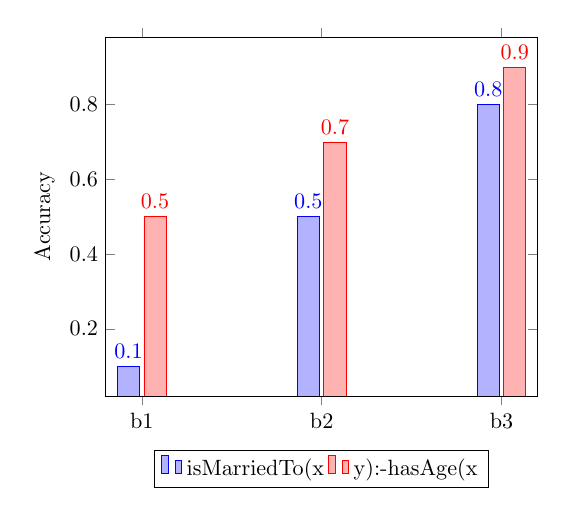
\begin{tikzpicture}[scale=0.8]
\begin{axis}[
    ybar,
    enlargelimits=0.10,
    legend style={at={(0.5,-0.15)},
      anchor=north,legend columns=-1},
    ylabel={Accuracy},
    symbolic x coords={b1,b2,b3},
    xtick=data,
    nodes near coords,
    nodes near coords align={vertical},
    ]
\addplot coordinates {(b1,0.1) (b2,0.5) (b3,0.8)};
\addplot coordinates {(b1,0.5) (b2,0.7) (b3,0.9)};
\legend{isMarriedTo(x,y):-hasAge(x,z) , isMarriedTo(x,y):-hasAge(x,z)hasChild(x,a)}
\end{axis}
\end{tikzpicture}
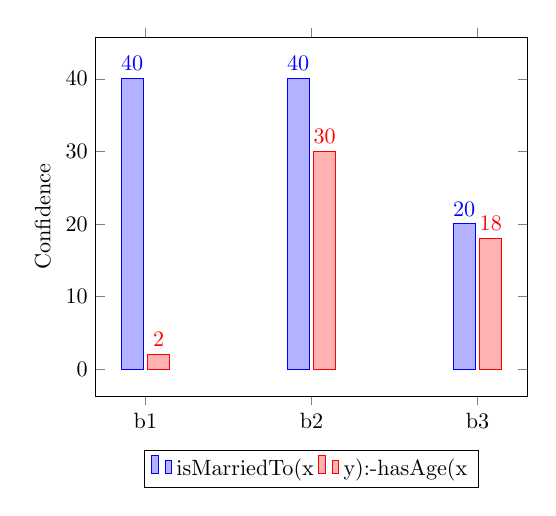
\begin{tikzpicture}[scale=0.8]
\begin{axis}[
    ybar,
    enlargelimits=0.15,
    legend style={at={(0.5,-0.15)},
      anchor=north,legend columns=-1},
    ylabel={Confidence},
    symbolic x coords={b1,b2,b3},
    xtick=data,
    nodes near coords,
    nodes near coords align={vertical},
    ]
\addplot coordinates {(b1,40) (b2,40) (b3,20)};
\addplot coordinates {(b1, 2) (b2,30) (b3,18)};
\legend{isMarriedTo(x,y):-hasAge(x,z) , isMarriedTo(x,y):-hasAge(x,z)hasChild(x,a)}
\end{axis}
\end{tikzpicture}

Adding some literals might not bring any gain or even loss in accuracy to the base-rule, but when bucketing per age, present a
different accuracy and support distribution and might even produce gain in accuracy for some specific buckets.

Nevertheless, adding a relation with no correlation to the rule might not generate any gain. Thus, it's necessary to carefully choose the relations and discard the uncorrelated ones.  

\section{Contributions}
In this Thesis, we propose a pre-processing step to build a graph we call \graphname for each numerical property we want to for interesting intervals. In each graph, that has a numerical property as root, we first query the examples distribution on the numerical attribute, and build a histogram by splitting them into \emph{k} buckets. Subsequently, we pick a set of \emph{c} categorical properties that can be joined with the root, extract the frequencies histogram and analyze how the distribution of sub-population created by joining them with the root is affected. Afterwards, we try to combine each of the categories and see if they still produce interesting sub-populations, like in frequent set
mining.

We discuss the pruning opportunities and also evaluate different heuristics and interestingness measures and their efficiency in finding rules with numerical intervals. 

\begin{comment}
In a clause containing a numerical attribute in the body, we can obtain a support and accuracy as well as support value
for each of the buckets. Therewith, we can search the most interesting intervals that satisfies the support and accuracy
thresholds
\end{comment}

With information about different examples distributions contained in the \graphname, once we add one of the root properties during the core ILP algorithm, we can then search for the most interesting categorical properties that could result in different accuracy distributions. For every categorical property we can also suggest the most interesting constants and other categorical properties to be combined in a subcategory of both.

\section{Outline}

\begin{comment}
 The remainder of this thesis is structured as follows. In
Chapter~\ref{ch:technical_background}, we provide technical background on
MapReduce and BigTable. In Chapter~\ref{ch:related_work}, we present a
summary of previous work in the areas of duplicate and near-duplicate detection,
information retrieval on web archives, and MapReduce applications in graph
processing. Following that, we state our problem and describe solutions in
Chapter~\ref{ch:redundancy_control}. In Chapter~\ref{ch:mapreduce_impl}, we
describe an implementation of our solution using the MapReduce framework. In
Chapter~\ref{ch:experiments}, we present our experimental results. We conclude
this thesis and outline directions of future research in Chapter~\ref{ch:future_work}.
\end{comment}
